% figure: 现控强化1-25-完整闭环结构图.png
\documentclass[border=10pt]{standalone}
\usepackage{fontspec}
\setmainfont{Cambria}
\usepackage{unicode-math}
\setmathfont{Cambria Math}
\usepackage{tikz}
\usetikzlibrary{arrows.meta,calc}
\begin{document}
\begin{tikzpicture}[>=Stealth,line width=.9pt,
 b/.style={draw,minimum width=1cm,minimum height=.7cm,fill=blue!4},
 s/.style={draw,circle,minimum size=.42cm,inner sep=0pt}]
\node[s] (u) at (0,0) {$+$};
\node[b] (bp) at (2,0) {$b$};
\node[s] (sp) at (4,0) {$+$};
\node[b] (ip) at (6,0) {$\dfrac{E_2}{s}$};
\node[b] (cp) at (9,0) {$c$};
\node[b] (ap) at (6,1.7) {$A$};
\node[b] (bo) at (2,-4) {$b$};
\node[s] (so) at (4,-4) {$+$};
\node[b] (io) at (6,-4) {$\dfrac{E_2}{s}$};
\node[b] (co) at (9,-4) {$c$};
\node[b] (ao) at (6,-2.3) {$A$};
\node[s] (err) at (11,-4) {$+$};
\node[b] (h) at (7,-5.8) {$h$};
\node[b] (k) at (1,-7.4) {$k$};
\draw[->] (-1.5,0) -- node[above] {$v$} (u);
\draw[->] (u) -- node[above] {$u$} (bp);
\fill (1,0) circle(1.4pt);
\draw[->] (1,0) |- (bo);
\draw[->] (bp) -- (sp);
\draw[->] (sp) -- node[above] {$\dot x$} (ip);
\draw[->] (ip) -- node[pos=.22,above] {$x$} (cp);
\fill (7.5,0) circle(1.4pt);
\draw[->] (7.5,0) |- (ap.east);
\draw[->] (ap.west) -| (sp.north);
\draw[->] (cp) -- node[above] {$y$} (12.5,0);
\fill (11,0) circle(1.4pt);
\draw[->] (11,0) -- (err.north);
\node at (11.32,-3.65) {$+$};
\draw[->] (bo) -- (so);
\draw[->] (so) -- node[above] {$\dot{\hat x}$} (io);
\draw[->] (io) -- node[pos=.22,above] {$\hat x$} (co);
\fill (7.5,-4) circle(1.4pt);
\draw[->] (7.5,-4) |- (ao.east);
\draw[->] (ao.west) -| (so.north);
\draw[->] (co) -- node[above] {$\hat y$} (err);
\node at (10.6,-4.28) {$-$};
\draw[->] (err.south) |- node[pos=.22,right] {$y-\hat y$} (h.east);
\draw[->] (h.west) -| (so.south);
\draw[->] (7.5,-4) -- (8,-4.7) -- (8,-7.4) -- (k.east);
\draw[->] (k.west) -- (0,-7.4) -- (u.south);
\node at (0.35,-.42) {$+$};
\node[anchor=north] at (6,-8.1) {$k=(-3,-4),\qquad h=(17/2,-1/2)^T$};
\end{tikzpicture}
\end{document}
